\documentclass[11pt]{article}
\usepackage[T1]{fontenc}
\usepackage{lmodern}
\usepackage{amsmath,amssymb}
\usepackage[margin=1in]{geometry}
\usepackage{graphicx,booktabs,microtype}
\usepackage[hidelinks]{hyperref}
\hypersetup{pdftitle={Cross-step interference, directional curvature, and gradient descent},
  pdfauthor={},pdfsubject={SGD formulation and full-batch CIFAR-10 GD evidence}}
\newcommand{\norm}[1]{\left\lVert#1\right\rVert}
\newcommand{\E}{\mathbb{E}}
\newcommand{\Loss}{\mathcal{L}}
\setlength{\parindent}{1.2em}
\setlength{\parskip}{3pt}
\setlength{\abovedisplayskip}{9pt}
\setlength{\belowdisplayskip}{9pt}
\setlength{\textfloatsep}{16pt}
\renewcommand{\arraystretch}{1.12}
\emergencystretch=1em
\title{Constructive and Destructive Training Regimes}
\author{}
\date{}

\begin{document}
\maketitle
\vspace{-2em}

\section{Introduction}

Training large language models (LLMs) relies on adaptive optimization, momentum, gradient clipping, learning-rate schedules and other heuristics to stabilize learning and mitigate undesired behavior such as loss spikes and oscillatory updates. Yet, despite their effectiveness, it is not fully understood why these mechanisms work, and under what conditions they fail.

To address this gap, we characterize a measurable, persistent behaviour of transition between two distinct learning regimes. Early in training, successive gradients tend to align, allowing updates to accumulate constructively as the loss decreases. Later, gradient directions reverse more frequently, causing successive updates to partially cancel one another. Despite this increased cancellation, the loss can continue to decrease.

Two complementary intuitions help explain this behavior. From the perspective of representation learning, each new mini-batch updates parameters that encode previously learned structure. Depending on its direction, an update may reinforce existing representations or partially undo them. From optimization geometry, a step may overshoot the bottom of a loss valley, prompting subsequent steps to reverse direction and partially retrace the path. Both mechanisms can give rise to oscillatory parameter updates even as optimization continues to make progress.

We formalize these dynamics using identities for stochastic gradient descent (SGD), connecting the alignment of consecutive gradients to curvature and gradient noise, and cumulative update cancellation to net parameter displacement. Building on these relations, we introduce scalable diagnostics to quantify and detect these dynamics and track the transition between constructive and oscillatory regimes during large-scale model training.


\section{Parameter displacement under stochastic gradient descent}

Let $\theta_t\in\mathbb{R}^p$ denote the parameters after update $t$, and let
$g_t$ denote a mini-batch gradient evaluated at $\theta_{t-1}$. We consider
a plain SGD with learning rate $\eta>0$, 
\begin{equation}
  \theta_t=\theta_{t-1}-\eta g_t.
  \label{eq:sgd}
\end{equation}
After $T$ updates, summing Eq.~\eqref{eq:sgd} gives the displacement from
initialization,
\begin{equation}
  \Delta_T:=\theta_T-\theta_0=-\eta\sum_{t=1}^T g_t.
  \label{eq:displacement}
\end{equation}
Expanding its squared norm separates individual gradient magnitudes from their
temporal interactions
\begin{equation}
  \norm{\Delta_T}^2
  =\eta^2\sum_{t=1}^T\norm{g_t}^2
   +2\eta^2\sum_{1\leq u<t\leq T}g_u^\top g_t.
  \label{eq:energy-interaction}
\end{equation}
The gradient-energy terms $\norm{g_t}^2$ are nonnegative. Each pairwise inner product
$g_u^\top g_t$ can be
positive, zero, or negative: aligned gradients reinforce their contribution to
the sum, whereas opposing gradients cancel part of it. 
To practically measure the alignement of nonzero consecutive gradients, define their cosine similarity as
\begin{equation}
  \rho_t:=\frac{g_{t-1}^\top g_t}{\norm{g_{t-1}}\norm{g_t}},
  \qquad t=2,\ldots,T.
  \label{eq:rho}
\end{equation}
Separating adjacent pairs from the remaining interactions yields
\begin{equation}
\begin{aligned}
\norm{\Delta_T}^2={}&\eta^2\sum_{t=1}^T\norm{g_t}^2\\
 &+2\eta^2\underbrace{\sum_{t=2}^T
    \norm{g_{t-1}}\norm{g_t}\rho_t}_{\text{lag-one interaction}}\\
 &+2\eta^2\underbrace{\sum_{t=3}^T\sum_{u=1}^{t-2}
    g_u^\top g_t}_{\text{interaction beyond lag one}}.
\end{aligned}
\label{eq:lag-split}
\end{equation}
Negative $\rho_t$ contributes cancellation between consecutive updates. However,
longer-lag interactions can reinforce or offset these negative contributions.
Thus, adjacent anti-alignment diagnoses a local interaction, while the complete
double sum determines longer-term cumulative interaction. 

\subsection{Curvature, gradient noise, and consecutive alignment}

For mini-batch SGD, we explicitly incorporate stochastic gradient noise and examine its contribution to their directional alignment. Let $\Loss$ denote the full training objective. We write a stochastic gradient
as
\begin{equation}
  g_t=\nabla\Loss(\theta_{t-1})+\xi_t,
  \label{eq:noise-model}
\end{equation}
where $\xi_t$ is the gradient estimation error. Suppose $\Loss$ is twice
continuously differentiable along the step under consideration, and define
$H_{t-1}:=\nabla^2\Loss(\theta_{t-2})$. Expanding the full gradient around
$\theta_{t-2}$ and substituting the preceding SGD step gives
\begin{equation}
  g_t=(I-\eta H_{t-1})g_{t-1}+(\xi_t-\xi_{t-1})+r_t,
  \label{eq:gradient-evolution}
\end{equation}
where $r_t$ is the Taylor remainder. Neglecting $r_t$ recovers the first-order
approximation. Taking the inner product with $g_{t-1}$ then gives
\begin{equation}
\rho_t\approx
\frac{
\underbrace{\|g_{t-1}\|^2}_{\text{Gradient magnitude}}
-
\underbrace{\eta g_{t-1}^{\top}H_{t-1}g_{t-1}}_{\text{Curvature contribution}}
+
\underbrace{g_{t-1}^{\top}(\xi_t-\xi_{t-1})}_{\text{Noise contribution}}
}{
\|g_{t-1}\|\|g_t\|
}.
\label{eq:rho-expanded}
\end{equation}
The numerator contains the preceding gradient energy, the curvature,
and the gradient noise contributions. Positive curvature along the preceding
gradient direction reduces its alignment with the next gradient. The noise
difference can reinforce or oppose this effect on an individual step. We normalize the curvature and noise terms by the preceding gradient energy
\begin{equation}
  \kappa_t:=\frac{g_{t-1}^\top H_{t-1}g_{t-1}}{\norm{g_{t-1}}^2},
  \qquad
  \varepsilon_t:=\frac{g_{t-1}^\top(\xi_t-\xi_{t-1})}
                            {\norm{g_{t-1}}^2}.
  \label{eq:kappa-epsilon}
\end{equation}
With these definitions, Eq.~\eqref{eq:rho-expanded} becomes
\begin{equation}
  \boxed{\rho_t\approx\frac{\norm{g_{t-1}}}{\norm{g_t}}
                   (1-\eta\kappa_t+\varepsilon_t).}
  \label{eq:rho-normalized}
\end{equation}
The norm ratio is positive, so the first-order sign prediction depends on
$1-\eta\kappa_t+\varepsilon_t$ (Table~\ref{tab:sign}). 

\begin{table}[htbp]
\centering
\caption{Consecutive-gradient alignment predicted by the first-order model.}
\label{tab:sign}
\begin{tabular}{lll}
\toprule
Alignment & Cosine sign & First-order condition\\
\midrule
Positive & $\rho_t>0$ & $\eta\kappa_t<1+\varepsilon_t$\\
Orthogonal & $\rho_t=0$ & $\eta\kappa_t=1+\varepsilon_t$\\
Negative & $\rho_t<0$ & $\eta\kappa_t>1+\varepsilon_t$\\
\bottomrule
\end{tabular}
\end{table}

% The remainder matters near this boundary. In fact,
% Eq.~\eqref{eq:gradient-evolution} implies the exact relation
% \begin{equation}
%   \rho_t=\frac{\norm{g_{t-1}}}{\norm{g_t}}
%           (1-\eta\kappa_t+\varepsilon_t+\delta_t),
%   \qquad
%   \delta_t:=\frac{g_{t-1}^\top r_t}{\norm{g_{t-1}}^2}.
%   \label{eq:remainder}
% \end{equation}
% The first-order sign is reliable only to the extent that this omitted term does
% not change the numerator's sign.

\subsubsection{Directional curvature}

The quantity $\kappa_t$ is a Hessian Rayleigh quotient along the preceding
stochastic gradient. If $H_{t-1}v_i=\lambda_i v_i$ in an orthonormal eigenbasis
and $g_{t-1}=\sum_i a_i v_i$, then
\begin{equation}
  \kappa_t=\frac{\sum_i\lambda_i a_i^2}{\sum_i a_i^2}.
  \label{eq:rayleigh}
\end{equation}
Thus, the gradient selects an eigenvalue-weighted average rather than the
maximum eigenvalue. A sharp direction can exist without contributing much to
the current gradient. Rearranging Eq.~\eqref{eq:rho-normalized} motivates the observable quantity
\begin{equation}
  \eta\widehat\kappa_t
  :=1-\rho_t\frac{\norm{g_t}}{\norm{g_{t-1}}}+\varepsilon_t.
  \label{eq:kappa-estimate}
\end{equation}
For mini-batch gradients, the noise term requires additional information and cannot
be recovered from adjacent cosine and norms alone. For full-batch GD, $\xi_t=0$ and hence $\varepsilon_t=0$. The recorded
gradient-only quantity is then exactly
\begin{equation}
\eta\widehat\kappa_t
 =1-\rho_t\frac{\norm{g_t}}{\norm{g_{t-1}}}
 =-\frac{g_{t-1}^\top(g_t-g_{t-1})}{\norm{g_{t-1}}^2}.
\label{eq:gd-proxy}
\end{equation}
It measures the change in the gradient projected onto its preceding direction.

\subsubsection{Noise contribution}

Under fresh, conditionally unbiased mini-batch sampling, we have
\begin{equation}
  \E[g_{t-1}^\top\xi_t]=0.
  \label{eq:fresh-noise}
\end{equation}
But because \(g_{t-1}\) already contains the previous noise \(\xi_{t-1}\), 
\begin{equation}
  \E[g_{t-1}^\top\xi_{t-1}]=\E[\norm{\xi_{t-1}}^2].
\end{equation}
Subtracting these two expectations yields
\begin{equation}
  \E[g_{t-1}^\top(\xi_t-\xi_{t-1})]
              =-\E[\norm{\xi_{t-1}}^2]\leq0.
  \label{eq:noise-expectation}
\end{equation}
Even unbiased noise therefore produces a nonpositive expected contribution to
the unnormalized adjacent inner product. It suggests a systematic mechanism through which stochastic gradient noise can reduce successive-gradient alignment, independently of the local directional curvature.

\subsection{Normalized displacement and cumulative interference}

Adjacent alignment concerns one pair of steps. To characterize accumulation
over the complete trajectory, we compare the sum of gradient lengths with the
length of their sum
\begin{equation}
  A_T:=\sum_{t=1}^T\norm{g_t},
  \qquad B_T:=\norm{\sum_{t=1}^T g_t}.
  \label{eq:ab}
\end{equation}
For Eq.~\eqref{eq:sgd}, $\eta A_T$ is the discrete path length and
$\eta B_T=\norm{\Delta_T}$ is its endpoint displacement. Provided $A_T>0$,
we define
\begin{equation}
  \boxed{R_T:=\frac{B_T}{A_T}
       =\frac{\norm{\Delta_T}}{\eta\sum_{t=1}^T\norm{g_t}}\in[0,1].}
  \label{eq:normalized-displacement}
\end{equation}
The numerator $B_T$ is the net displacement; the denominator $A_T$ is the total length of all SGD steps. This normalized displacement $R_T$ expresses how much of the accumulated step length remains as net motion of parameters after the gradient directions reinforce or cancel one another. 

\subsection{Full-batch GD evidence on CIFAR-10}

We examine the small CIFAR-10 squared-loss setting used in the released
edge-of-stability experiments~\cite{cohen2021,eoscode}. We use the first 5,000 CIFAR-10 training images and a fully connected
$3072$--$200$--$200$--$10$ network with tanh hidden activations and biases
($656{,}810$ parameters). Four GD runs share
the same frozen initialization from seed zero and use learning rates
\(
  \eta\in\{0.004,2/300,0.01,0.02\}.
\)
Each run completes 20,000 updates with no momentum, weight decay,
clipping, augmentation, learning-rate schedule, or injected gradient noise. We record loss and raw-gradient diagnostics at every update. The largest
Hessian eigenvalue is estimated on all 5,000 examples at initialization
and every 100 updates. Figure~\ref{fig:gd} shows all recorded values. 

\begin{figure}[htbp]
  \centering
  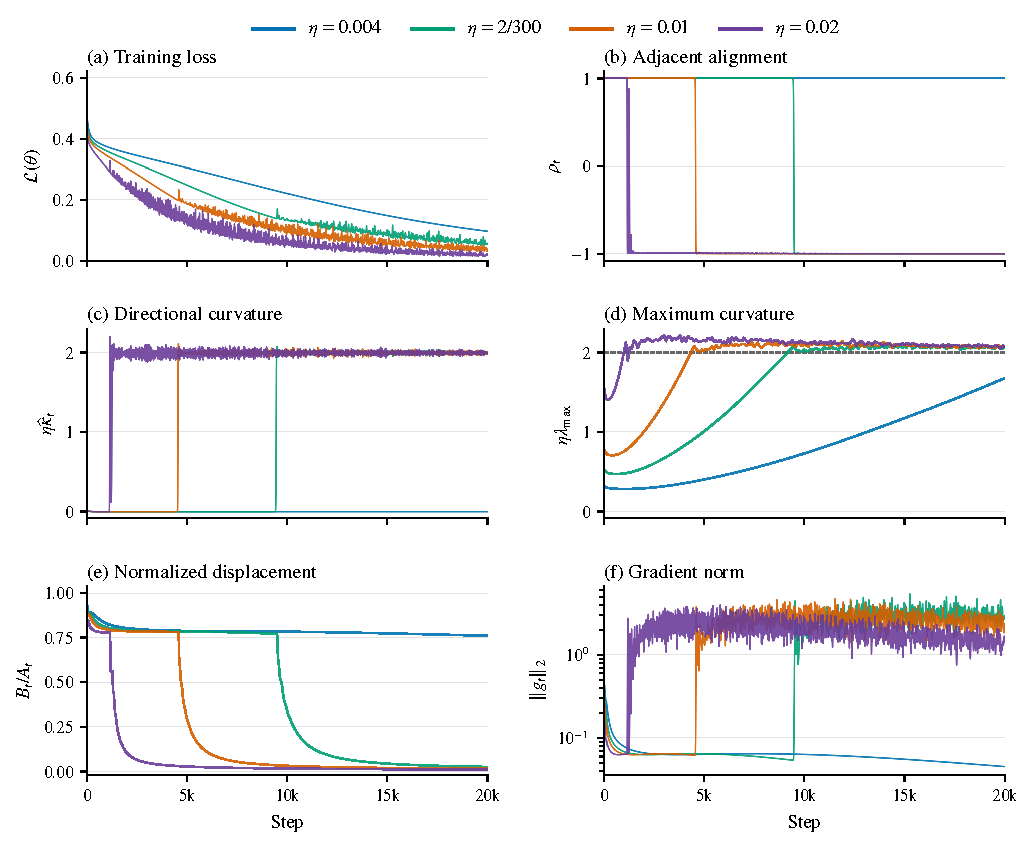
\includegraphics[width=\linewidth]{../../analyses/019-2026-10-13-cifar10-eos-lr/figures/cifar10_gd_diagnostics_paper.pdf}
  \caption{Full-batch GD on CIFAR-10 with four matched learning rates.
  (a) Training loss; (b) consecutive-gradient cosine;
  (c) the gradient-derived quantity
  $\eta\widehat\kappa_t=1-\rho_t\norm{g_t}/\norm{g_{t-1}}$;
  (d) the scaled largest algebraic Hessian eigenvalue, with the dashed reference
  at two; (e) full-prefix normalized displacement $B_t/A_t$; and
  (f) raw-gradient norm on log Y. All curves are unsmoothed.
  Hessians are measured every 100 updates; the other diagnostics are measured
  every update. Larger learning rates enter the alternating-gradient regime
  earlier. Loss decreases over the horizon while cumulative cancellation and
  oscillatory gradient magnitudes increase.}
  \label{fig:gd}
\end{figure}

\clearpage

Figure~\ref{fig:gd} shows that larger learning rates lead to an earlier
transition from constructive to destructive interference between consecutive
updates (panel~b). This transition is accompanied by a sharp rise and peak in
the estimated directional curvature $\eta\widehat\kappa_t$ (panel~c), with
$\eta\lambda_{\max}$ (panel~d) near the critical GD scale of two. The
correspondence between these curvature diagnostics links the observed
transition to the high-curvature spectral regime in these runs. The
accompanying abrupt drop of $B_t/A_t$ toward zero (panel~e) shows that most of
the accumulated path length is cancelled, leaving only a small fraction as
net parameter displacement. Finally, gradient norms grow and fluctuate
(panel~f), a behavior that our current formulation of alignment and
displacement does not explain.

\paragraph{TODO: an alignment-guided learning-rate intervention.}
Test a schedule that halves the learning rate when consecutive-gradient cosine
becomes negative, specifying the trigger and repeat rule before execution.
Compare loss reduction at a matched update budget with fixed-rate controls.
The intervention may restore positive alignment without improving convergence;
these two outcomes must be evaluated separately.

\section{Extending the SGD formulation to momentum}

For Adam with constant learning rate $\eta>0$ and no weight decay,
\begin{equation}
  \theta_t=\theta_{t-1}-\eta d_t,
  \qquad d_t:=\frac{\widehat m_t}{\sqrt{\widehat v_t}+\epsilon},
  \label{eq:adam-update}
\end{equation}
where the operations in $d_t$ are elementwise and
\begin{equation}
\begin{aligned}
  m_t&=\beta_1m_{t-1}+(1-\beta_1)g_t,
  &\widehat m_t&=\frac{m_t}{1-\beta_1^t},\\
  v_t&=\beta_2v_{t-1}+(1-\beta_2)g_t^{\odot2},
  &\widehat v_t&=\frac{v_t}{1-\beta_2^t}.
\end{aligned}
\label{eq:adam-moments}
\end{equation}
Here $m_0=v_0=0$, $\beta_1,\beta_2\in[0,1)$, and $\epsilon>0$.
The displacement expansion becomes
\begin{equation}
  \norm{\Delta_T}^2=\eta^2\sum_{t=1}^T\norm{d_t}^2
       +2\eta^2\sum_{1\leq u<t\leq T}d_u^\top d_t.
  \label{eq:adam-displacement}
\end{equation}
Although $d_t$ determines parameter displacement, we study the stored first
moment $m_t$ to separate temporal gradient coherence from adaptive
preconditioning. Gradients still evolve along the actual Adam trajectory.

\subsection{Consecutive-momentum alignment}

For nonzero momentum norms and $t\geq2$, the recurrence gives the exact identity
\begin{equation}
  c_t:=\frac{m_{t-1}^\top m_t}{\norm{m_{t-1}}\norm{m_t}}
  =\frac{\beta_1\norm{m_{t-1}}^2+(1-\beta_1)m_{t-1}^\top g_t}
         {\norm{m_{t-1}}\norm{m_t}}.
  \label{eq:momentum-cosine}
\end{equation}
Using the earlier gradient-noise notation, a first-order expansion along
the Adam step, neglecting the Taylor remainder, yields
\begin{equation}
  g_t\approx g_{t-1}-\eta H_{t-1}d_{t-1}+(\xi_t-\xi_{t-1}).
  \label{eq:adam-gradient-evolution}
\end{equation}
Define the momentum-tracking, curvature and noise contributions as
\begin{equation}
\begin{aligned}
  a_t&:=\frac{m_{t-1}^\top(g_{t-1}-m_{t-1})}{\norm{m_{t-1}}^2},\\
  \kappa_t^{(m)}&:=\frac{m_{t-1}^\top H_{t-1}d_{t-1}}{\norm{m_{t-1}}^2},\\
  \varepsilon_t^{(m)}&:=\frac{m_{t-1}^\top(\xi_t-\xi_{t-1})}{\norm{m_{t-1}}^2}.
\end{aligned}
\label{eq:momentum-contributions}
\end{equation}
Substitution into Eq.~\eqref{eq:momentum-cosine} gives
\begin{equation}
  \boxed{c_t\approx\frac{\norm{m_{t-1}}}{\norm{m_t}}
  \left[1+(1-\beta_1)
  \left(a_t-\eta\kappa_t^{(m)}+\varepsilon_t^{(m)}\right)\right].}
  \label{eq:momentum-alignment-model}
\end{equation}
The factor $1-\beta_1$ scales these contributions to alignment.
Unlike SGD, $\kappa_t^{(m)}$ is generally not a Hessian Rayleigh quotient:
$m_{t-1}$ and the preconditioned direction $d_{t-1}$ need not be parallel.

\subsection{Normalized momentum accumulation}

With $A_T^{(m)}:=\sum_{t=1}^T\norm{m_t}>0$ and
$B_T^{(m)}:=\norm{\sum_{t=1}^T m_t}$, define
\begin{equation}
  \boxed{R_T^{(m)}:=\frac{B_T^{(m)}}{A_T^{(m)}}
  =\frac{\norm{\sum_{t=1}^T m_t}}{\sum_{t=1}^T\norm{m_t}}\in[0,1].}
  \label{eq:momentum-accumulation}
\end{equation}
Values near one indicate reinforcement; smaller values indicate cumulative
cancellation. This describes momentum accumulation, while Adam displacement
depends on $d_t$. Bias correction leaves $c_t$ unchanged but generally changes
the cumulative ratio, so accumulation of $m_t$ and $\widehat m_t$ must be
distinguished.

\clearpage
\section{Controlled Rosenbrock experiments}

We compare three deterministic AdamW trajectories on
$f(x,y)=(1-x)^2+100(y-x^2)^2$, whose minimum is $(1,1)$.
All runs start at $(0,1)$ and perform 2,000 float64 updates at
$\eta\in\{10^{-2},10^{-2.5},10^{-3}\}$, with
$(\beta_1,\beta_2)=(0.9,0.95)$, $\epsilon=10^{-8}$, weight decay $0.1$,
and exact gradients. With zero gradient noise, rearranging
Eq.~\eqref{eq:momentum-alignment-model} gives the momentum estimate
\begin{equation}
\begin{aligned}
  \eta\widehat\kappa_t^{(m)}
  &:=a_t+\frac{1-c_t\norm{m_t}/\norm{m_{t-1}}}{1-\beta_1}\\
  &=\frac{m_{t-1}^\top(g_{t-1}-g_t)}{\norm{m_{t-1}}^2}.
\end{aligned}
\label{eq:momentum-curvature-estimate}
\end{equation}
Both gradient-derived estimates follow the AdamW trajectory; adaptive updates,
decay and finite-step effects prevent identifying them with $\lambda_{\max}$.
All paths enter the curved valley and approach the minimum
(Fig.~\ref{fig:rosenbrock-trajectories}). Larger learning rates reach
raw-gradient reversal earlier, whereas momentum remains positively aligned
on average (Fig.~\ref{fig:rosenbrock-diagnostics}). Cumulative $B/A$ stays high:
late reversal therefore need not imply substantial cancellation over the
full trajectory. The smallest learning rate attains the lowest final objective.

\begin{figure}[htbp]
  \centering
  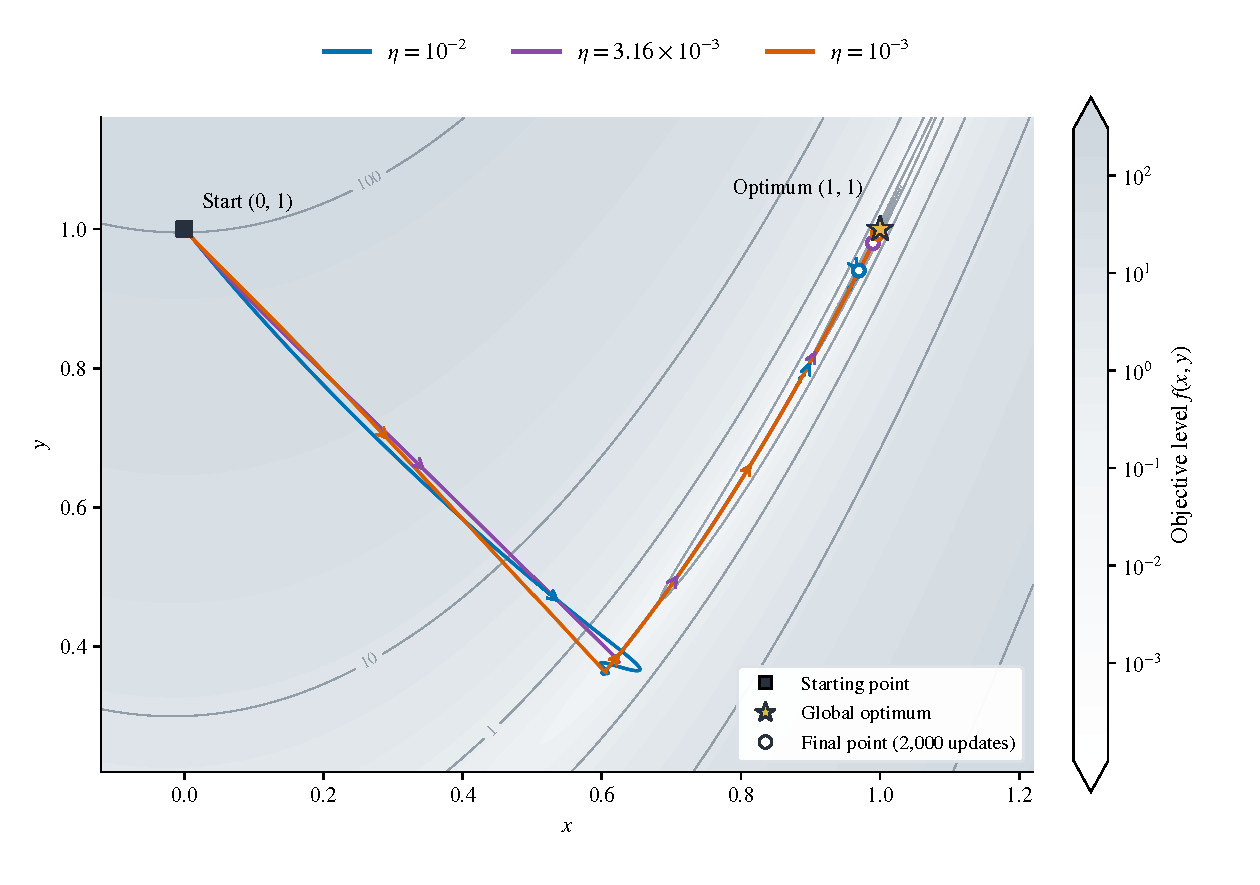
\includegraphics[width=\linewidth]{../../analyses/017-2026-10-12-rosenbrock-kappa-identity/figures/rosenbrock_trajectories_paper.pdf}
  \caption{Complete AdamW trajectories on Rosenbrock objective level curves.
  The square and star mark the common start and global minimum; circles mark
  final states. Arrows follow update order.}
  \label{fig:rosenbrock-trajectories}
\end{figure}

\begin{figure}[p]
  \centering
  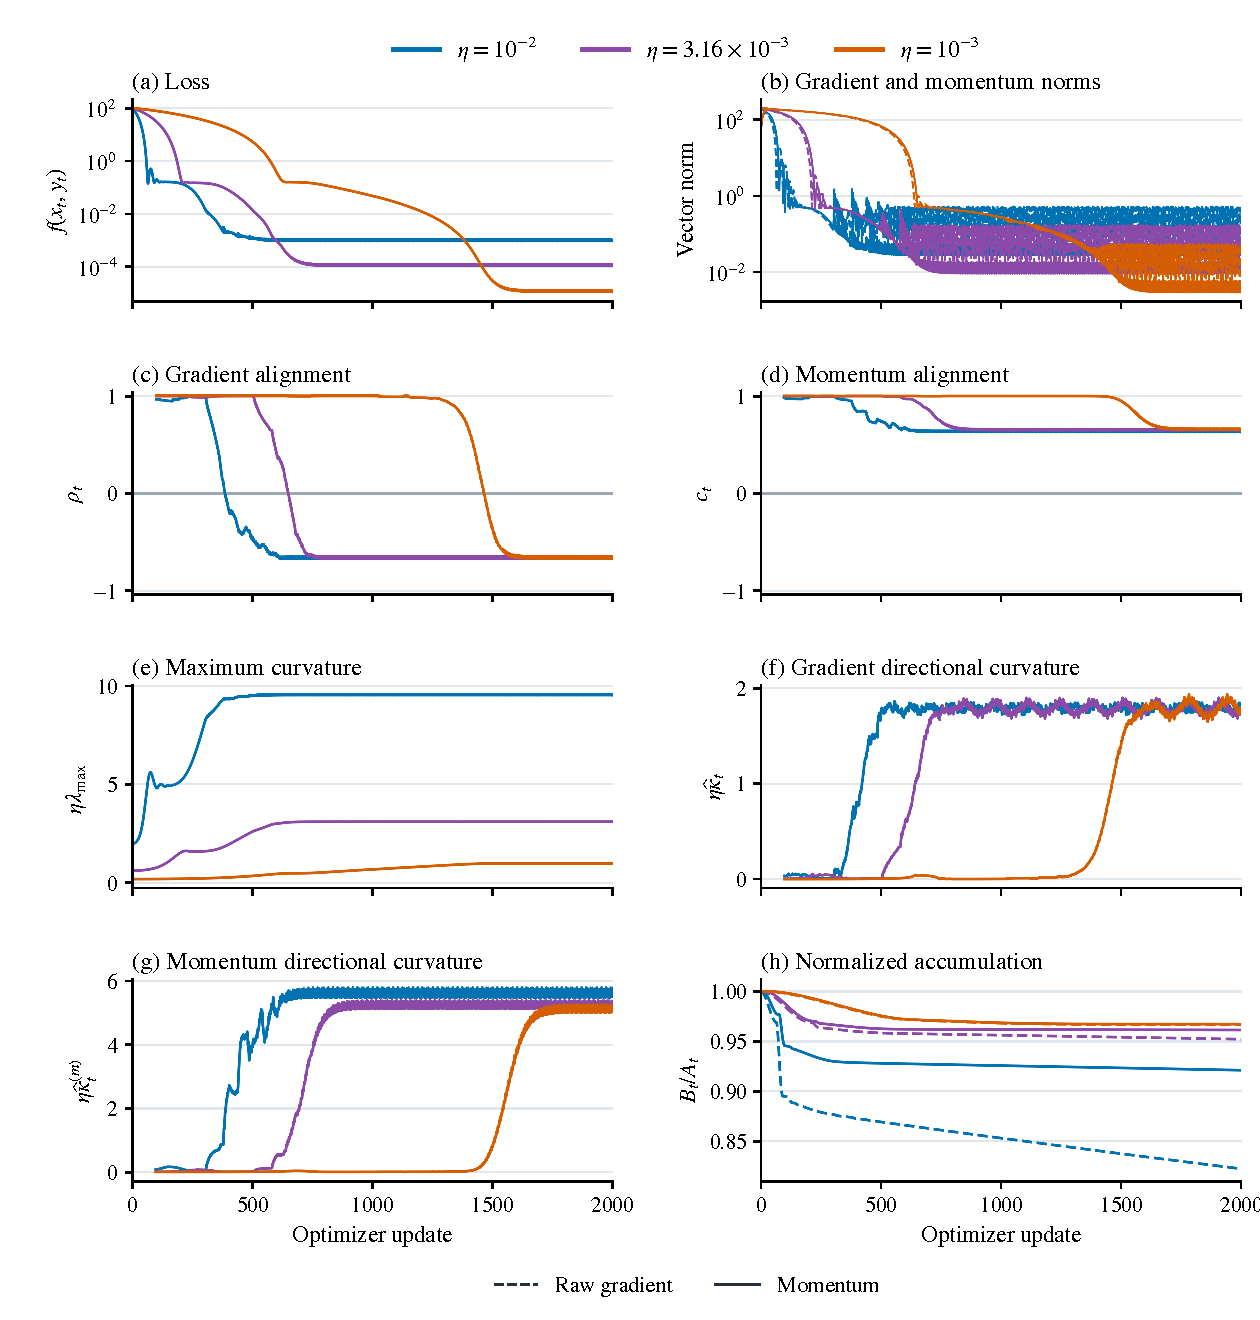
\includegraphics[width=\linewidth]{../../analyses/017-2026-10-12-rosenbrock-kappa-identity/figures/rosenbrock_diagnostics_paper.pdf}
  \caption{Rosenbrock diagnostics for the three learning rates.
  (a) Objective; (b) raw-gradient and stored-momentum norms (log Y);
  (c,d) adjacent cosines; (e) $\eta\lambda_{\max}$;
  (f,g) gradient- and momentum-derived curvature estimates;
  (h) full-prefix $B/A$, with raw gradients dashed.
  Panels (c,d,f,g) use complete 100-pair trailing means, first defined at
  update 101; other curves are unsmoothed. All 2,000 updates are retained.}
  \label{fig:rosenbrock-diagnostics}
\end{figure}
\clearpage

\subsection{Gradient-estimation noise}

We repeat the same setup with $g_t=\nabla f(\theta_{t-1})+\xi_t$, where
$\xi_t\sim\mathcal N(0,\sigma^2 I_2)$ and
$\sigma\in\{0,0.01,0.1,1,10\}$. One seed (1234) supplies shared
standard-normal draws across noise levels and learning rates; $\sigma=0$
is the deterministic control. In this paired realization, stronger noise
raises the objective and reduces raw-gradient $B/A$, while momentum
remains positively aligned on average (Fig.~\ref{fig:rosenbrock-noise}).

\begin{figure}[htbp]
  \centering
  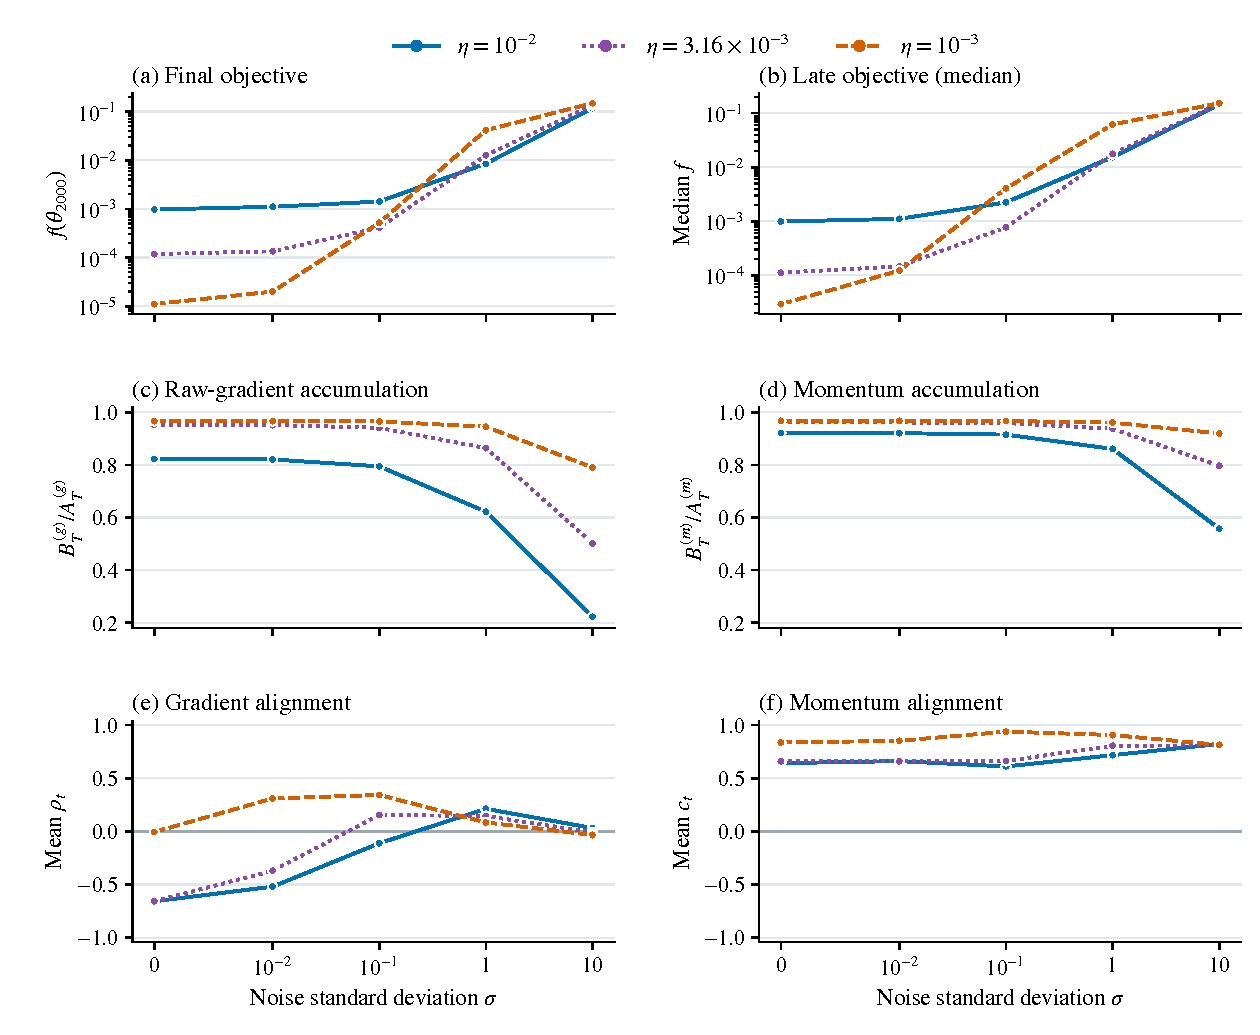
\includegraphics[width=\linewidth]{../../analyses/014-2026-10-10-rosenbrock-gradient-noise/figures/sigma_comparison_paper.pdf}
  \caption{Gaussian gradient-noise sweep. (a) Final objective; (b) median
  objective over the last 1,000 updates; (c,d) full-prefix $B/A$ for noisy
  gradients and stored momentum; (e,f) mean unsmoothed adjacent cosine over
  updates 1,001--2,000. Each marker is one trajectory; lines connect sampled
  noise levels. Objective uses log Y; the $\sigma$ axis is symmetric log,
  linear through $0.01$. One paired seed; no uncertainty bands.}
  \label{fig:rosenbrock-noise}
\end{figure}
\clearpage

\begin{thebibliography}{9}
\bibitem{cohen2021}
J.~M.~Cohen, S.~Kaur, Y.~Li, J.~Z.~Kolter, and A.~Talwalkar.
\newblock Gradient descent on neural networks typically occurs at the edge of
stability.
\newblock \emph{International Conference on Learning Representations}, 2021.
\newblock \url{https://arxiv.org/abs/2103.00065}.

\bibitem{eoscode}
J.~M.~Cohen and collaborators.
\newblock Released implementation of the edge-of-stability experiments,
\texttt{github} branch.
\newblock \url{https://github.com/locuslab/edge-of-stability/tree/github}.
\end{thebibliography}
\end{document}
